
\documentclass[10pt]{article}
\usepackage[utf8]{inputenc}
\usepackage{kotex}
\usepackage{graphicx}
\usepackage{subfigure}
\usepackage{titling}
\setlength{\droptitle}{-2cm}
\usepackage{array}
\usepackage{amssymb}
\usepackage{amsmath}
\usepackage{siunitx} 
\usepackage{enumerate} 
\usepackage{pgfplots}
\usepackage{pgfplotstable}
\usepackage{tikz,pgfplots}
\usepackage{wasysym}
\usepackage{geometry}
\usepackage{authblk}
\usepackage{kotex}
\usepackage{bibunits}
\usepackage{tabularx}
\usepackage{hyperref}
\usepackage{pythonhighlight}

\geometry{
    a4paper,
    total={170mm,257mm},
    left=20mm,
    top=20mm,
}

\title{\textbf{Mathematical Foundation of DNN : HW 9}}
\author{Jeong Min Lee}

\begin{document}
\maketitle

\section*{1}

\begin{figure}[!h]
    \begin{center}
        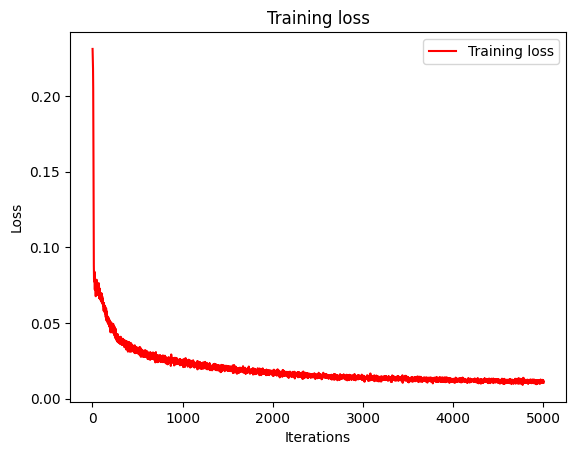
\includegraphics[scale = 0.5]{fig/fig1.png}
    \end{center}
    \caption{The training loss of the autoencoder. }
    \label{fig1}
\end{figure}

As the figure \ref{fig1} depicts, the training of autoencoder was success. 
The calculated threshold from the validation dataset was about 23.6706.
In the test dataset, the rate of score function exceeding the threshold in MNIST and KMNIST dataset was observed.
For MNIST test dataset, the null hypothesis is that the classifier correctly identifies all MNIST images within the test set as non-anomalies so that the examples whose score function exceeding the threshold are included in type I error. 
For KMIST test dataset, the null hypothesis is that the classifier correctly identifies all KMNIST images as anomalies so that the examples whose score function lower than the threshold become instances of type II error. 
As a result, the type I error is 0.009, while type II error is 0.0286. 


\section*{2}
\begin{figure}[!h]
    \begin{center}
        \subfigure[]{
            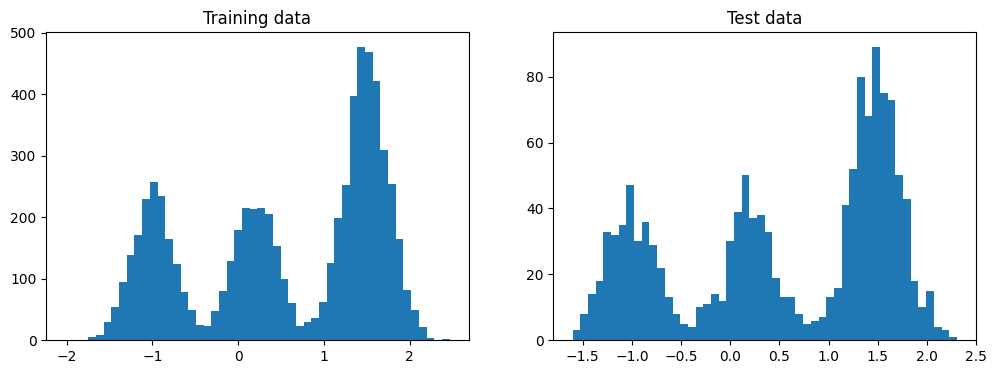
\includegraphics[scale = 0.5]{fig/fig2.png}
        }
        \subfigure[]{
            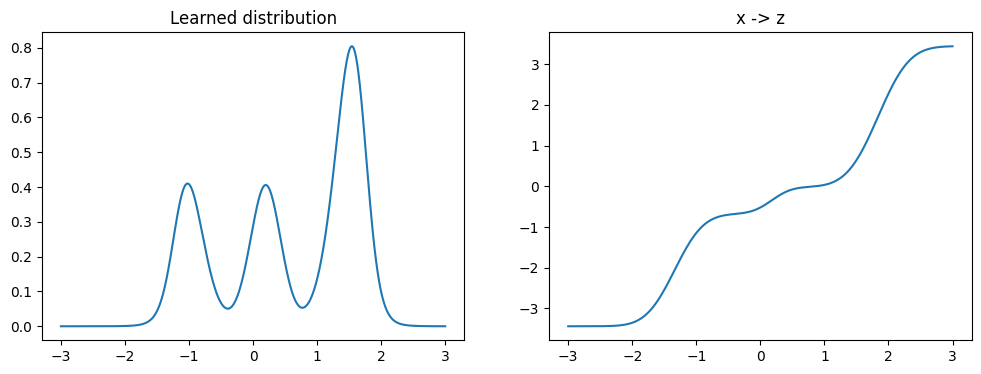
\includegraphics[scale = 0.5]{fig/fig4.png}
        }
        \subfigure[]{
            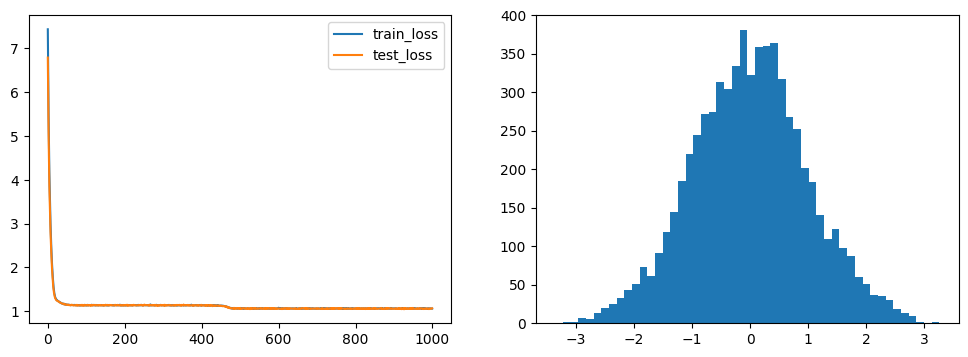
\includegraphics[scale = 0.5]{fig/fig3.png}
        }
    \end{center}
    \caption{(a) The distribution of training data and test data. (b) The learned distribution from training dataset (left) and the flow from $x$ to $z$ (right). (c) The training loss and test loss of the model (left) and the empirical distribution of $z$ (right)}
    \label{fig2}
\end{figure}

To solve this problem, the example source code of chapter 5 was slightly changed.
As the example code does, several plots that visualize the training process of model and model's output. 
As the figures \ref{fig2}(c) illustrates, the training of the model was success and the empirical distribution of $z$ resembled to the target distribution, $\mathcal{N}(0,1)$
\clearpage

\section*{3}
Let $P_\sigma$ be the permutation matrix that maps $x = P_\sigma \begin{pmatrix} x_\Omega \\ x_{\Omega^c}\end{pmatrix}$. In addition, for same permutation matrix $P_\sigma$, $z = P_\sigma \begin{pmatrix} z_\Omega \\ z_{\Omega^c}\end{pmatrix}$, by definition.
Then,
\begin{align*}
    {\partial z \over \partial x} &= \begin{pmatrix}
        {\partial z^{(1)} \over \partial x^{(1)}} & \cdots & {\partial z^{(1)} \over \partial x^{(n)}} \\
        \vdots & \ddots & \vdots \\
        {\partial z^{(n)} \over \partial x^{(1)}} & \cdots & {\partial z^{(n)} \over \partial x^{(n)}}
    \end{pmatrix} \\
    &= P_\sigma^{-1} \begin{pmatrix}
        {\partial z_\Omega \over \partial x_\Omega} & {\partial z_\Omega \over \partial x_{\Omega^c}} \\
        {\partial z_{\Omega^c} \over \partial x_\Omega} & {\partial z_{\Omega^c} \over \partial x_{\Omega^c}}
    \end{pmatrix}P_\sigma \\
    &= P_\sigma^{-1} \begin{pmatrix}
        I & 0 \\ \star & \text{diag}(e^{s_\theta(x_\Omega)})
    \end{pmatrix}P_\sigma
\end{align*}
Note that the permutation matrices are multiplied infront and behind of the upper triangular matrix since the rows and columns of original matrix are exchanged in same manner.
Considering the properties of determinant,
\begin{align*}
    \log\left(\det {\partial z \over \partial x}\right) &= \log\left(\det(\text{diag}(e^{s_\theta(x_\Omega)}))\right)\\
    &= \log \left(\prod_{i=1}^{n - |\Omega|} {e^{s_\theta(x_\Omega)}}^{(i)}\right) \\
    &= \sum_{i=1}^{n - |\Omega|} s_\theta (x_\Omega)^{(i)}\\
    &= \mathbf{1}_{{n - |\Omega|}}^Ts_\theta (x_\Omega)
\end{align*}
\section*{4}
\subsection*{a}
\begin{align*}
    D_{KL}(X|Y) &= \mathbb{E}_X\left[\log\left(X/Y\right)\right] \\
    &= \mathbb{E}_X\left[-\log(Y/X)\right]\\
    &\ge -\log\left(\mathbb{E}_X[Y/X]\right) \; (\because \text{ Jensen's inequality})\\
    &= -\log\left(\int_{\mathbb{R}^d} f(x)\frac{g(x)}{f(x)} dx \right) \\
    &= -\log 1 \; \left(\because \int_{\mathbb{R}^d} g(x) dx = 1 \right)\\
    &= 0
\end{align*}
\subsection*{b}
Since $X_i$ are random variable, $X$ is random vector. $\mathbf{X}$ is used to emphasize that $X$ is random vector.
Since $X_i$ are independent, by definition, its PDF $f_{\mathbf{X}}(\mathbf{x}) = f_{X_1}(x_1) \times \cdots \times f_{X_d}(x_d)$ for some sample vector $\mathbf{x}$. 
Thus, it is natural to represent $D_{KL}$ as follows. 
\begin{align*}
    D_{KL}(\mathbf{X}|\mathbf{Y}) &= \int_{\mathbb{R}^d} f_{\mathbf{X}}(\mathbf{x})\log\frac{f_{\mathbf{X}}(\mathbf{x})}{g_{\mathbf{Y}}(\mathbf{x})} d\mathbf{x}\\
    &= \int_{\mathbb{R}^d}f_{X_1}(x_1) \times \cdots \times f_{X_d}(x_d)\left( \log\frac{f_{X_1}(x_1)}{g_{Y_1}(x_1)} + \cdots + \log\frac{f_{X_d}(x_d)}{g_{Y_d}(x_d)}\right) dx_1\cdots dx_d \\
    &= \int_{\mathbb{R}}f_{X_1}(x_1)\log\frac{f_{X_1}(x_1)}{g_{Y_1}(x_1)}dx_1\int_{\mathbb{R}}f_{X_2}(x_2)dx_2 \cdots \int_{\mathbb{R}}f_{X_d}(x_d) dx_d + \\ 
    &\cdots + \int_{\mathbb{R}}f_{X_1}(x_1)dx_1 \int_{\mathbb{R}} f_{X_2}(x_2)dx_2 \cdots \int_{\mathbb{R}}f_{X_d}(x_d)\log\frac{f_{X_d}(x_d)}{g_{Y_d}(x_d)}dx_d \\
    &= \int_{\mathbb{R}}f_{X_1}(x_1)\log\frac{f_{X_1}(x_1)}{g_{Y_1}(x_1)}dx_1 + \cdots + \int_{\mathbb{R}}f_{X_d}(x_d)\log\frac{f_{X_d}(x_d)}{g_{Y_d}(x_d)}dx_d \\
    &= D_{KL}(X_1|Y_1) + \cdots + D_{KL}(X_d|Y_d)
\end{align*}

\section*{5}
\begin{align*}
    &D_{KL}(\mathcal{N}(\mu_0, \Sigma_0)|\mathcal{N}(\mu_1, \Sigma_1)) \\
    &= \int_{\mathbb{R}^d} d\mathbf{x} \frac{1}{\sqrt{(2\pi)^d}}(\det{\Sigma_0})^{-1/2}\exp\left(-\frac{1}{2}\mathbf{(x - \mu_0)}^T\Sigma_0^{-1}\mathbf{(x-\mu_0)}\right)\\ &\times \left[\log\left(\frac{\det \Sigma_0^{-1/2}}{\det \Sigma_1^{-1/2}}\right) - \frac{1}{2}(\mathbf{x - \mu_0})^T\Sigma_0^{-1}\mathbf{(x-\mu_0)} + \frac{1}{2}\mathbf{(x-\mu_1)}^T\Sigma_1^{-1}(\mathbf{x-\mu_1})\right] \\
    &= \log\left(\frac{\det \Sigma_0^{-1/2}}{\det \Sigma_1^{-1/2}}\right)\int_{\mathbb{R}^d} d\mathbf{x} \frac{1}{\sqrt{(2\pi)^d}}(\det{\Sigma_0})^{-1/2}\exp\left(-\frac{1}{2}\mathbf{(x - \mu_0)}^T\Sigma_0^{-1}\mathbf{(x-\mu_0)}\right) \\
    & -\frac{1}{2}\int_{\mathbb{R}^d} d\mathbf{x} \frac{1}{\sqrt{(2\pi)^d}}(\det{\Sigma_0})^{-1/2}\exp\left(-\frac{1}{2}\mathbf{(x - \mu_0)}^T\Sigma_0^{-1}\mathbf{(x-\mu_0)}\right)(\mathbf{x - \mu_0})^T\Sigma_0^{-1}\mathbf{(x-\mu_0)} \\
    & + \frac{1}{2}\int_{\mathbb{R}^d} d\mathbf{x} \frac{1}{\sqrt{(2\pi)^d}}(\det{\Sigma_0})^{-1/2}\exp\left(-\frac{1}{2}\mathbf{(x - \mu_0)}^T\Sigma_0^{-1}\mathbf{(x-\mu_0)}\right)(\mathbf{x - \mu_1})^T\Sigma_1^{-1}\mathbf{(x-\mu_1)} \\
    &= \frac{1}{2}\log\frac{\det \Sigma_1}{\det \Sigma_0}-\frac{1}{2}\int_{\mathbb{R}^d} d\mathbf{x} \frac{1}{\sqrt{(2\pi)^d}}(\det{\Sigma_0})^{-1/2}\exp\left(-\frac{1}{2}\mathbf{(x - \mu_0)}^T\Sigma_0^{-1}\mathbf{(x-\mu_0)}\right)(\mathbf{x}^T\Sigma_0^{-1}\mathbf{x} - 2\mathbf{\mu}_0^T\Sigma_0^{-1}\mathbf{x} + \mathbf{\mu}_0^T\Sigma_0^{-1}\mathbf{\mu}_0) \\ 
    &+ \int_{\mathbb{R}^d} d\mathbf{x} \frac{1}{\sqrt{(2\pi)^d}}(\det{\Sigma_0})^{-1/2}\exp\left(-\frac{1}{2}\mathbf{(x - \mu_0)}^T\Sigma_0^{-1}\mathbf{(x-\mu_0)}\right)(\mathbf{x}^T\Sigma_1^{-1}\mathbf{x} - 2\mathbf{\mu}_1^T\Sigma_1^{-1}\mathbf{x} + \mathbf{\mu}_1^T\Sigma_1^{-1}\mathbf{\mu}_1)\\
    &= \frac{1}{2}\log\frac{\det \Sigma_1}{\det \Sigma_0} -\frac{1}{2}\mathbb{E}\left[X^T\Sigma_0^{-1}X - 2\mu_0^T\Sigma_0^{-1}X + \mu_0^T\Sigma_0^{-1}\mu_0\right] + \frac{1}{2}\mathbb{E}\left[X^T\Sigma_1^{-1}X - 2\mu_1^T\Sigma_1^{-1}X + \mu_1^T\Sigma_1^{-1}\mu_1\right] \\ 
    &= \frac{1}{2}\log\frac{\det \Sigma_1}{\det \Sigma_0} - \frac{1}{2}\left(\mathbb{E}[X^T\Sigma_0^{-1}X] - \mathbf{\mu}_0^T\Sigma_0^{-1}\mathbf{\mu}_0\right) + \frac{1}{2}\left(\mathbb{E}[X^T\Sigma_1^{-1}X] - 2\mathbf{\mu}_1^T\Sigma_1^{-1}\mathbf{\mu}_0 + \mathbf{\mu}_1^T\Sigma_1^{-1}\mathbf{\mu}_1\right) \\
    &= \frac{1}{2}\left[\log\frac{\det \Sigma_1}{\det \Sigma_0} - \mathbb{E}[X^T\Sigma_0^{-1}X] + \mathbb{E}[X^T\Sigma_1^{-1}X] + (\mu_1 - \mu_0)^T \Sigma_1^{-1}(\mu_1 - \mu_0) - \mu_0^T(\Sigma_1^{-1} - \Sigma_0^{-1})\mu_0\right]
\end{align*}
\begin{align*}
    \mathbb{E}\left[X^TA X\right] &= \mathbb{E}\left[\text{tr}(X^TAX)\right] \\
    &= \mathbb{E}\left[\text{tr}(AXX^T)\right]\\
    &= \text{tr}\left(A\mathbb{E}[XX^T]\right) \; (\because \text{ mean and trace operator are linear operator.})\\
    &= \text{tr}\left(A(\Sigma + \mu\mu^T)\right) \\
    &= \text{tr}\left(A\Sigma + A\mu\mu^T\right) \\
    &= \text{tr}(A\Sigma) + \text{tr}(\mu^TA\mu) \\
    &= \text{tr}(A\Sigma) + \mu^TA\mu
\end{align*}

By inserting $A = \Sigma_0$ in the equation above, $\mathbb{E}[X^T\Sigma_0^{-1}X] = \text{tr}(\Sigma_0^{-1}\Sigma_0) + \mu_0^T\Sigma_0^{-1}\mu_0 = d + \mu_0^T\Sigma_0^{-1}\mu_0$. Likewise, by inserting $A = \Sigma_1$, $\mathbb{E}[X^T\Sigma_1^{-1}X] = \text{tr}(\Sigma_1^{-1}\Sigma_0) + \mu_0^T\Sigma_1^{-1}\mu_0$.
Thus, putting both terms into the $D_{KL}(\mathcal{N}(\mu_0, \Sigma_0)|\mathcal{N}(\mu_1, \Sigma_1))$, the proof is done.
\begin{align*}
    D_{KL}(\mathcal{N}(\mu_0, \Sigma_0)|\mathcal{N}(\mu_1, \Sigma_1)) &= \frac{1}{2}\left[\log\frac{\det \Sigma_1}{\det \Sigma_0} + (\mu_1 - \mu_0)^T\Sigma_1^{-1}(\mu_1 - \mu_0) - d + \text{tr}\left(\Sigma_1^{-1}\Sigma_0\right)\right] 
\end{align*}
\section*{6}
To be clear, the following property is used rather the the one given by hint: $\max_{\theta,\phi}g(\theta,\phi) = \max_{\theta}\left(\max_{\phi}g(\theta,\phi)\right)$.
To prove it, $M_1 \equiv \max_{\theta,\phi}g(\theta,\phi), M_2 \equiv \max_{\theta}\left(\max_{\phi}g(\theta,\phi)\right)$.
First of all, consider $M_1  = g(\theta^\star, \phi^\star)$ where $\theta^\star \in \Theta, \phi^\star \in \Phi$.
Then, for fixed $\theta \in \Theta$, $g(\theta, \phi^\star) \le \max_\phi g(\theta, \phi)$. 
Thus, $M_1 = g(\theta^\star,\phi^\star) \le \max_\phi g(\theta^\star, \phi) \le \max_\theta(\max_\phi g(\theta,\phi)) = M_2$.
On the other hand, let $\phi^\star = \arg\max_\phi g(\theta,\phi)$. Then, $M_1 = \max_{\theta, \phi} g(\theta, \phi) \ge \max_\theta g(\theta, \phi^\star) = \max_\theta(\max_\phi g(\theta, \phi))$. Thus, $M_1 = M_2$.


By using the property proved above, the following discussion is possible. 
\begin{align*}
    \max_{\theta,\phi} g(\theta, \phi) &= \max_{\theta}(\max_{\phi}g(\theta,\phi)) \\
    &= \max_\theta(\max_\phi f(\theta) - h(\theta, \phi))\\
    &= \max_\theta(f(\theta) - \min_\phi h(\theta, \phi)) \\
    &= \max_\theta f(\theta)
\end{align*}

Therefore, 
\begin{align*}
    \left\{\theta \bigg| (\theta, \phi) \in \arg\max_{\theta, \phi}g(\theta, \phi)\right\} &= \left\{\theta \bigg| g(\theta, \phi) = \max_{\theta, \phi}g(\theta, \phi)\right\} \\
    &= \left\{\theta \bigg| g(\theta,\phi) = \max_{\theta}f(\theta) \text{ with } h(\theta, \phi) = 0\right\} \\
    &= \left\{\theta \bigg| f(\theta, \phi) = \max_{\theta}f(\theta)\right\} \\
    &= \arg\max_{\theta}f
\end{align*}

\end{document}